\setlength{\columnsep}{3pt}
\begin{flushleft}
\bigskip
\paragraph{What is a CPU cores?}

\begin{itemize}
	\item A “core” is a single CPU. 
	\item A CPU core is a physical hardware component.	
\end{itemize}


\bigskip
\paragraph{What is a CPU thread?}
\begin{itemize}
	\item A core can be virtually splitted into parts called \textbf{thread}.
	\item A core uses threads to offer more power to specific programs.
	\item A thread virtually divides one CPU core into 2 parts giving the effect of 2 cores.
	\item A thread implements \textbf{hyperthreading} which is responsible for multi-tasking.
\end{itemize}

\begin{figure}[h!]
	\centering
	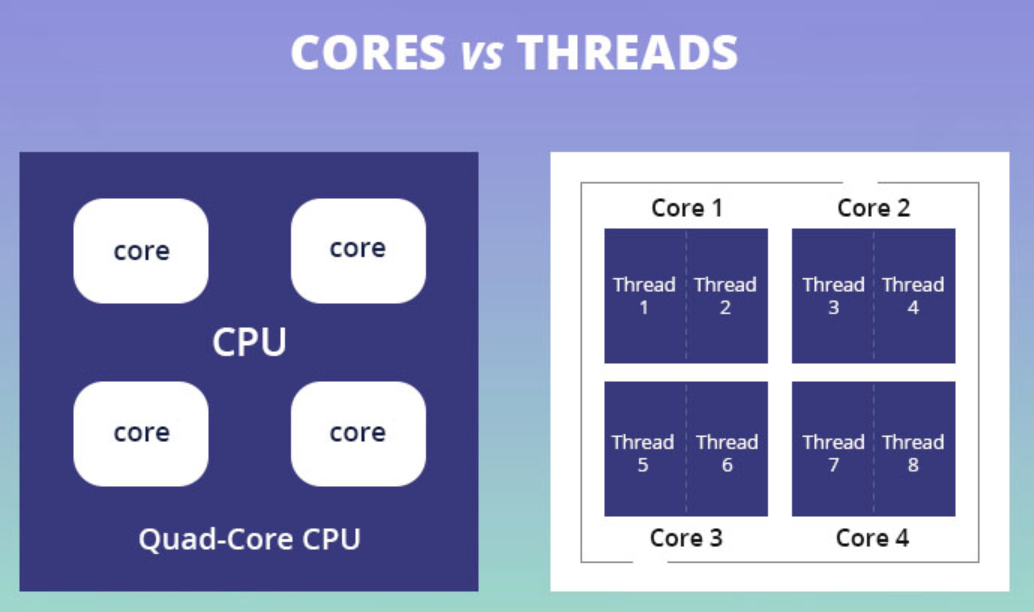
\includegraphics[scale=.3]{content/chapter12/images/core.png}
	\caption{Core \& Thread}
	\label{fig:process3}
\end{figure}



\end{flushleft}

\newpage


